\documentclass[10pt]{book}

\usepackage{cdt/cdtUsecases}
\usepackage{txfonts}


% !TeX root = proyecto.tex

% Encabezados y pie de página
\fancyhead[LE]{
\includegraphics[height=35pt]{theme/headerPar}} 
\fancyhead[RO]{
\includegraphics[height=35pt]{theme/headerInp}} 
\fancyhead[RE]{} 
\fancyhead[LO]{} 

\fancyfoot[CO,CE]{{\tiny\color{subTitleColor}\em Av. Juan de Dios Bátiz esq. Miguel Othón de Mendizabal S/N Col. Lindavista, GAM, D. F. {\color{sectionColor}\Telefon} 57296000 Ext. 52004 {\color{sectionColor}\Letter} ulises.velez@gmail.com}}
\fancyfoot[RO,LE]{\footnotesize\thepage}


%=========================================================
% Datos del documento:
\defProyecto{Nombre del sistema o proyecto}
\defNumComponente{Componente 2}
\defComponente{Documento de análisis}
\defEtapa{Etapa del documento: etapa 1, iteración 5, sprint 4, etc.}

%=========================================================
% Datos de la consultora:
\defConsultora{Nombre de la consultora}
\defNomSupervisor{Nombre del responsable por parte de la consultora}
\defCargoSupervisor{Cargo del responsable de la consultora: Líder de proyecto, Scrum Master, Project Manager, etc.}

%=========================================================
% Datos del cliente:
\defCliente{Nombre de la empresa cliente}
\defNomResponsable{Nombre del responsable del proyecto por parte de la empresa}
\defCargoResponsable{Cargo del responsable de la empresa}

\title{\Proyecto\bigskip\\\Componente}
\subtitle{\Etapa}
\author{\Consultora}
\organization{\Cliente}
\showInstrucciones
\date{\color{red}Borrador Fecha de creación de documento\\(para revisión)}

%\date{\color{green}Version 1.0}

%%%%%%%%%%%%%%%%%%%%%%%%%%%%%%%%%%%%%%%%%%%%%%%%%%%%%%%%%%%%%%%%
\begin{document}
\renewcommand{\listtablename}{Índice de tablas}
\renewcommand{\tablename}{Tabla} 
\ThisLRCornerWallPaper{1}{theme/bannerAzul}
\maketitle
\thispagestyle{empty}

\frontmatter
\tableofcontents
\listoffigures
\listoftables

% !TeX root = proyecto.tex

%=========================================================
%\chapter{Project Charter}

\newcommand{\ESCOMPchSec}[1]{\rowcolor{colorAgua}\multicolumn{4}{|c|}{\bf #1}\\\hline}
\newcommand{\ESCOMPchItem}[2]{{\bf {#1}} & \multicolumn{3}{p{.66\textwidth}|}{#2}\\\hline}
\newcommand{\ESCOMPchSubItem}[3]{{\bf {#1}} & {#2} & \multicolumn{2}{p{.44\textwidth}|}{#3}\\\hline}
\newcommand{\ESCOMPchSubSubItem}[4]{{\bf {#1}} & {#2} & {#3}& {#4}\\\hline}

\cleardoublepage
{\centering{\Huge Project Charter}\bigskip\\}
\begin{table}[hptb!] 
%\renewcommand\thetable{i}
\begin{tabular}{|p{.22\textwidth} |p{.22\textwidth} |p{.22\textwidth} |p{.22\textwidth} |}
	\hline
	\ESCOMPchItem{Proyecto:}{CVE, Nombre proyecto.}
	\ESCOMPchItem{Responsable:}{Empresa, Nombre del responsable, cargo, Firma.}
	\ESCOMPchItem{Autoriza:}{Empresa, Nombre del responsable, cargo, Firma.}
	\ESCOMPchItem{Background/Contexto:}{Descripción breve del contexto, no mas de 3 líneas.}
	\ESCOMPchItem{Beneficios esperados:}{Principales beneficios al término del proyecto.}
	\ESCOMPchItem{Costo estimado:}{\$ 2,350,700.00 $\pm$ 13\% (por ejemplo.)}
	\ESCOMPchSubSubItem{Fecha de inicio:}{Fecha}{\bf Fecha de término:}{Fecha.}
	\ESCOMPchItem{Objetivo:}{Objetivo general del proyecto.}
	\ESCOMPchSec{Entregables Principales}
	\ESCOMPchSubItem{}{Clave-Nombre}{descripción del entregable}
	\ESCOMPchSubItem{}{Clave-Nombre}{descripción del entregable}
	\ESCOMPchSubItem{}{...}{}
	\ESCOMPchSec{Alcance del proyecto}
	\ESCOMPchItem{Incluye:}{
		\begin{Titemize}
			\Titem Elemento 1 del alcance que incluye.
			\Titem ...
		\end{Titemize}
	}
	\ESCOMPchItem{Excluye:}{
		\begin{Titemize}
			\Titem Elemento 1 del alcance que incluye.
			\Titem ...
		\end{Titemize}
	}
	\ESCOMPchItem{Criterio de éxito:}{Indicador clave de término del proyecto}
	\ESCOMPchItem{Metodología:}{Metodología o metodologías que se utilizan (dos renglones o lista de no mas de 7)}
	\ESCOMPchSec{Datos de contacto}
	\ESCOMPchItem{Project Manager:}{Nombre, Tel, correo, etc.}
	\ESCOMPchItem{Project owner:}{Nombre, Tel, correo, etc.}
	\ESCOMPchItem{...}{}
	\ESCOMPchItem{Riesgos y peligros:}{
		\begin{Titemize}
			\Titem Riesgo o peligro identificado.
			\Titem ...
		\end{Titemize}
	}
	\ESCOMPchItem{Supuestos:}{
		\begin{Titemize}
			\Titem Suposiciones hechas de las que depende el éxito del proyecto.
			\Titem ...
		\end{Titemize}
	}
	\ESCOMPchItem{Restricciones y dependencias:}{
		\begin{Titemize}
			\Titem Restricciones del proyecto.
			\Titem ...
		\end{Titemize}
	}
	\ESCOMPchSec{Supervisión}
	\ESCOMPchSubItem{Juntas:}{(Nombre de la(s) persona(s)),}{ reporta a (Nombre de la(s) persona(s))}
	\ESCOMPchSubItem{Dudas:}{(Nombre de la(s) persona(s)),}{ reporta a (Nombre de la(s) persona(s))}
	\ESCOMPchSubItem{Avances:}{(Nombre de la(s) persona(s)),}{ reporta a (Nombre de la(s) persona(s))}
	\ESCOMPchSubItem{...}{}{}
\end{tabular}
	\caption{Resumen del proyecto}
	\label{tbl:projectCharter}
\end{table}


\mainmatter
\LRCornerWallPaper{1}{theme/pleca}

%%%%%%%%%%%%%%%%%%%%%%%%%%%%%%%%%%%%%%%%%%%%%%%%%%%%%%%%%%%%%%%%

%=========================================================
% !TeX root = proyecto.tex

%=========================================================
\chapter{Introducción}


\cdtInstrucciones{
	Presentar el documento, indicando su contenido, a quien va dirigido, quien lo realizó, por que razón, dónde y cuando. \\
}
	Este documento contiene el análisis de requerimientos del proyecto ``{\em Nombre del proyecto}'' que servirá como base para el análisis, diseño, construcción, pruebas y aceptación del proyecto.

%---------------------------------------------------------
\section{Presentación}


\cdtInstrucciones{
	Presente en un par de párrafos el contexto y el problema en que se define el proytecto.
}

\cdtInstrucciones{
	Indique el propósito del documento, a quien va dirigido y como debe ser utilizado el documento.
}
	
%---------------------------------------------------------
\section{Organización del contenido}

\cdtInstrucciones{
	Indique el contenido y organización del documento.
}
	En el capítulo \ref{cap:reqUsr} ...
	
	En el capítulo \ref{cap:reqSist} ...

%---------------------------------------------------------
\section{Notación, símbolos y convenciones utilizadas}

\cdtInstrucciones{
	Indique la notacion utilizada así como nórmas o estándares de documentación utilizados en el documento.
}	



%=========================================================
% !TeX root = proyecto.tex

%=========================================================
\chapter{Modelo del alcance}
\label{cap:alcance}

\cdtInstrucciones{
	Indique un resumen que describa el contenido del capítulo.
}
	
%---------------------------------------------------------
\section{Análisis de la problemática}

\cdtInstrucciones{
	Indique en un párrafo o dos el contenido y organización de la problemática.
}
% - - - - - - - - - - - - - - - - - - - - - - - - - - - - 
\subsection{Contexto del proyecto}

\cdtInstrucciones{
	Indique los antecedentes, contexto y características relevantes necesarios para comprender la problemática a resolver.
}

% - - - - - - - - - - - - - - - - - - - - - - - - - - - - 
\subsection{Problemas identificados}

\cdtInstrucciones{
	Describa el problema general y realice una lista con los problemas específicos a resolver mediante el proyecto.
}
El problema general que atiende el presente proyecto es: 


\begin{quotation}
	{\em ``Descripción de la problemática generar''}
\end{quotation}

Los problemas identificados son\FootnotePrioridad

%\begin{problemas}
%   \problema{P-01}{Nombre problema}{Descripción del problema}{A}
%   \problema{P-02}{Nombre del problema}{Descripción}{M}
%   \problema{...}{...}{...}{...}
%\end{problemas}
 
% - - - - - - - - - - - - - - - - - - - - - - - - - - - - 
\subsection{Análisis de causas probables}

\cdtInstrucciones{
	Describa las posibles causas de los problemas señalados.
}
\begin{description}
	\item[P-01] Describa una de las posibles causas de la problemática.
	\item[...] ...
\end{description}

% - - - - - - - - - - - - - - - - - - - - - - - - - - - - 
\subsection{Análisis de posibles consecuencias}

\cdtInstrucciones{
	Describa las consecuencias inmediatas, a mediano y largo plazo si la problemática persiste.
}
\begin{description}
	\item[P-01] Describa una de las posibles consecuencias de la problemática.
	\item[...] ...
\end{description}
 
% - - - - - - - - - - - - - - - - - - - - - - - - - - - - 
\subsection{Características de la solución}

\cdtInstrucciones{
	Describa los componentes, características, ideas o herramientas que integran la propuestas de solución.
}

Para atender la problemática anterior se propone implementar las siguientes acciones.

\begin{description}
	\item[P-01] Describa la solución propuesta para atender el problema P-01 explicando de qué forma lo resuelve.
	\item[P-02] ...
\end{description}

% - - - - - - - - - - - - - - - - - - - - - - - - - - - - 
\subsection{Síntesis de la problemática}

\cdtInstrucciones{
	Redacte las conclusiones del análisis de la problemática. Explique de manera general la solución o sistema a realizar a manera de propuesta y los beneficios que se obtendrán al implementar la solución.
}

%---------------------------------------------------------
\section{Objetivos del proyecto}

% - - - - - - - - - - - - - - - - - - - - - - - - - - - - 
\subsection{Objetivo general}

\cdtInstrucciones{
	Redacte el objetivo general del proyecto de la forma:\\
	VERBO EN INFINITIVO + (LO QUE SE VA A REALIZAR CON 2 O 3 CARACTERÍSTICAS RELEVANTES) + ``para'' + PROBLEMA QUE RESUELVE + ``mediante'' + 2 O 3 CARACTERÍSTICAS RELEVANTES DE LA SOLUCIÓN.
}

\begin{quotation}
	{\em ``Objetivo''}
\end{quotation}

% - - - - - - - - - - - - - - - - - - - - - - - - - - - - 
\subsection{Objetivos específicos}

\cdtInstrucciones{
	Liste los objetivos específicos adoptando el enfoque que más se adapte a su proyecto: por etapas, de lo general a lo específico, señalando componentes o partes de la solución, etc.
}

\begin{itemize}
	\item...
\end{itemize}


%---------------------------------------------------------
\section{Usuarios identificados}

\cdtInstrucciones{
	Coloque un diagrama a manera de organigrama en donde se indiquen quienes serán usuarios del sistema. 
}

\begin{figure}[htbp!]
	\begin{center}
		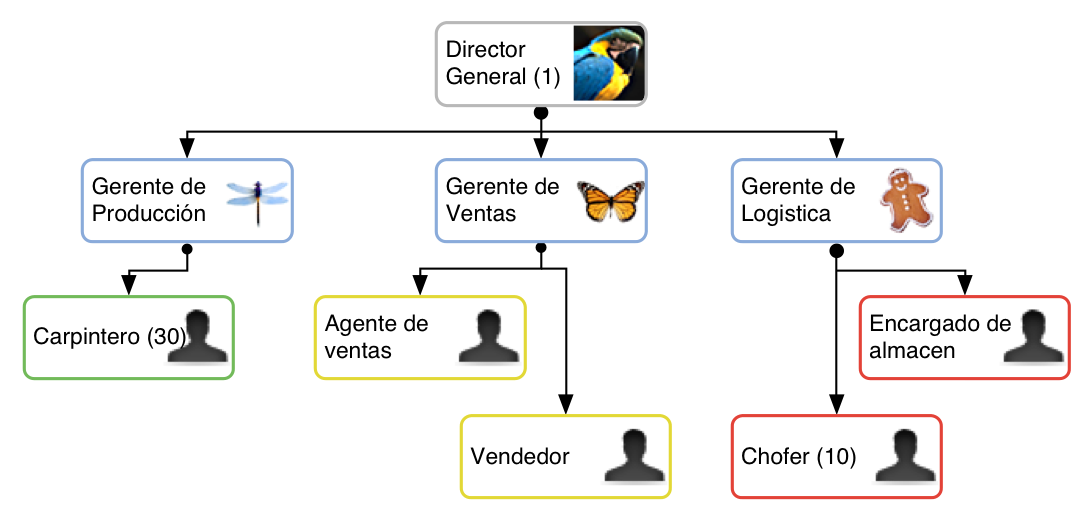
\includegraphics[width=.8\textwidth]{images/organigramaEm}
		\caption{Organigrama de la Mueblería Qetzal S. A. de C. V.}
		\label{fig:organigrama}
	\end{center}
\end{figure}


%---------------------------------------------------------
\section{Procesos involucrados}

\cdtInstrucciones{
	Coloque el mapa de procesos de la organización y liste a continuación los proceso que serán afectados por el desarrollo del sistema. Para cada proceso indique: Clave, Nombre y descripción.
}

\begin{figure}[htbp!]
	\begin{center}
		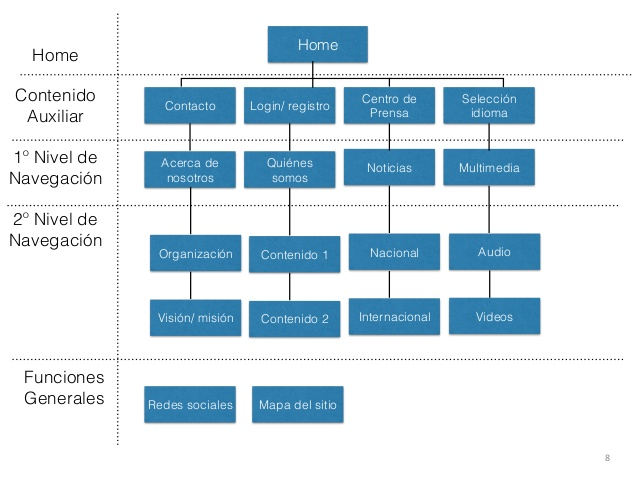
\includegraphics[width=.8\textwidth]{images/mapa}
		\caption{Mapa de procesos de la Mueblería Qetzal S. A. de C. V.}
		\label{fig:mapaProcASIS}
	\end{center}
\end{figure}

\begin{description}
	\item[PR-01] Nombre del proceso. Descripción del proceso.
\end{description}

%---------------------------------------------------------
\section{Requerimientos de usuario}

\cdtInstrucciones{
	Identifique y describa los requerimientos del usuario señalando: id, nombre, descripción y prioridad.
}

Los requerimientos del usuario son los siguientes\FootnoteStatus:

%\begin{requerimientosU}
%	\FRitem{RU-01}{Nombre del requerimiento}{Descripción del requerimiento.}{1}{\TODO}
%	\FRitem{...}{...}{...}{...}{...}
%\end{requerimientosU}

%---------------------------------------------------------
\section{Especificación de plataforma}	

\cdtInstrucciones{
	Coloque un diagrama y su descripción para aclarar el tipo de solución propuesta. \\
	
 En esta sección se debe aclarar:
	
\begin{description}
	\item[Tipo de sistema:] Web, aplicación móvil, de escritorio, híbrida, etc.
	\item[Software requerido:] Programas que se deberán instalar, desde el sistema operativo, compiladores, interpretes, servidores, etc.
	\item[Hardware requerido:] CPU, núcleos, velocidad, memoria, disco duro, etc.
	\item[servicios:] De conexión, seguridad, firewall, respaldo de energía, redundancia, uso de raids, etc.
\end{description}
}

\begin{figure}[htbp!]
	\begin{center}
		\fbox{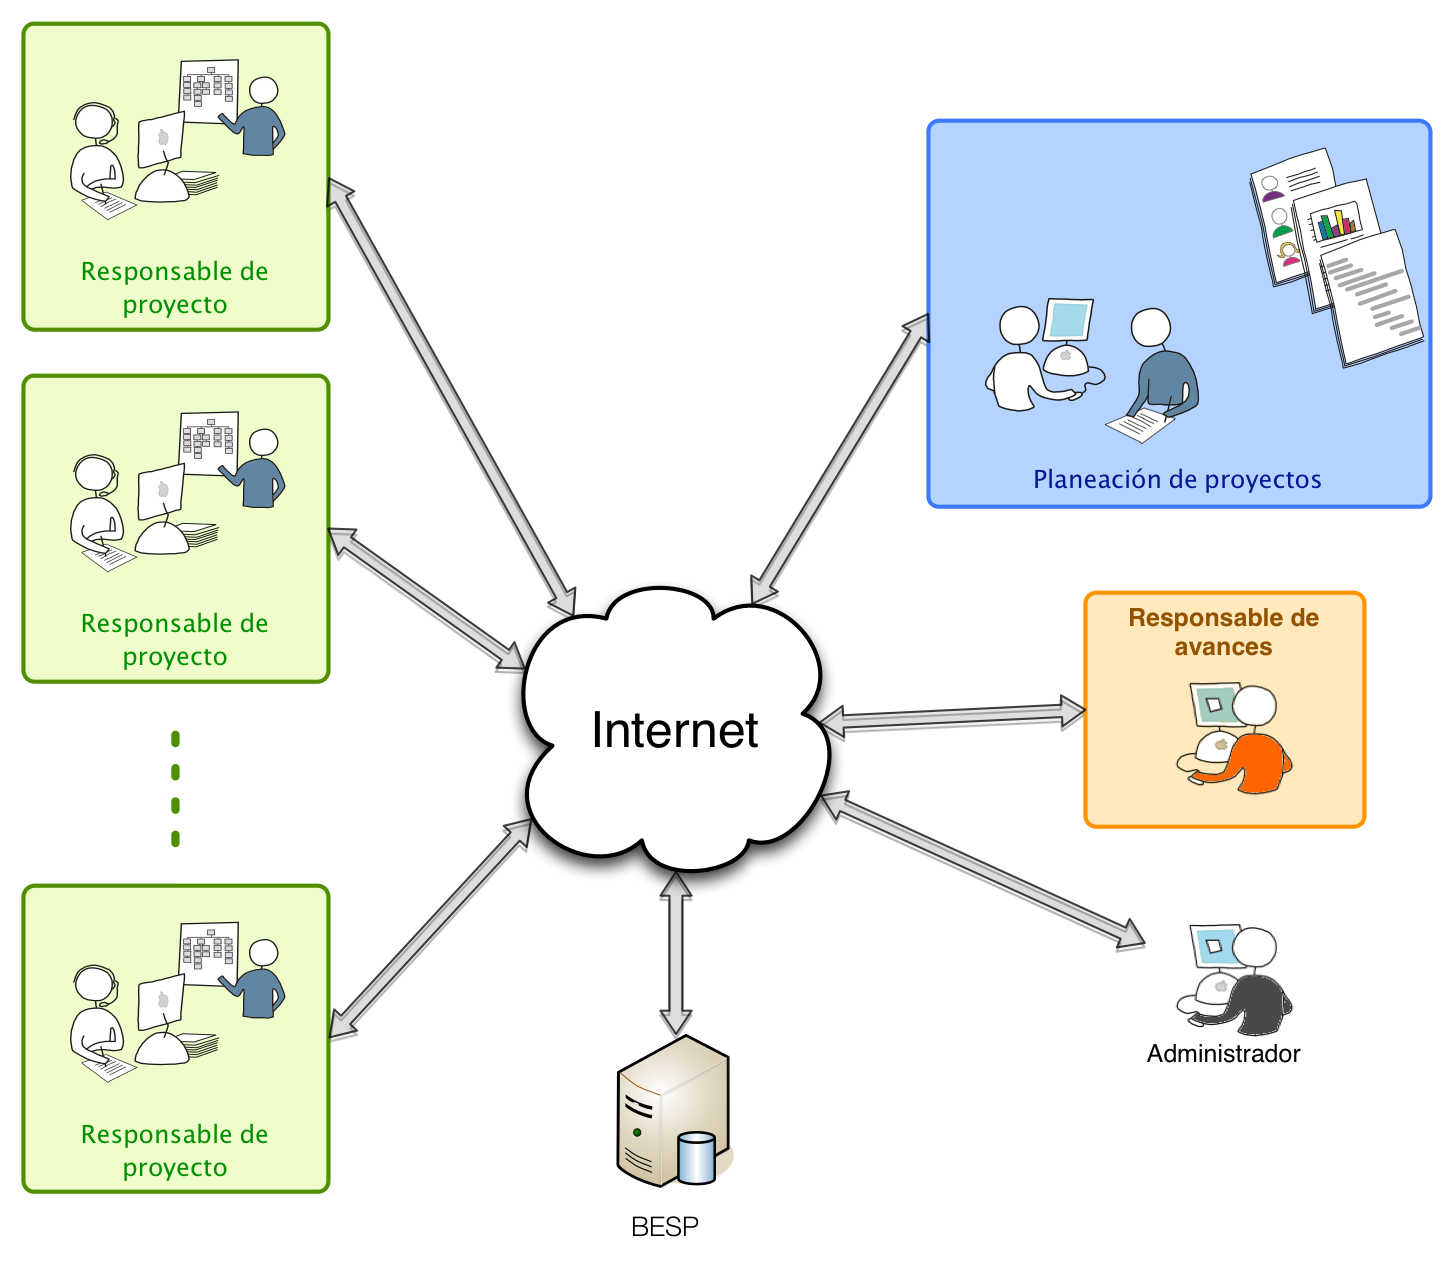
\includegraphics[width=.6\textwidth]{images/arquitectura}}
		\caption{Arquitectura del sistema.}
		\label{fig:arquitectura}
	\end{center}
\end{figure}

En la figura~\ref{fig:arquitectura} se describe la estructura del sistema, en ella se detalla ...




%=========================================================
% !TeX root = proyecto.tex

%=========================================================
\chapter{Modelo del Negocio}	
\label{cap:reqSist}

\cdtInstrucciones{Introduzca el capítulo describiendo el contenido del mismo, su organización y propósito.}

%----------------------------------------------------------
\section{Actores del sistema}

	\cdtInstrucciones{En esta sección describa a los actores del sistema.}
	
	%---------------------------------------------------------
	\begin{Usuario}{\hypertarget{A.NombreDelUsuario}{\subsection{Nombre del usuario}}}{
			Descripción del usuario: su puesto
		}
		\item[Responsabilidades:] \cdtEmpty
		\begin{itemize}
			\item Listar todas las responsabilidades y actividades dentro de la empresa.
			\item ...
		\end{itemize}
		
		\item[Perfil:] \cdtEmpty
		\begin{itemize}
			\item Describa el perfil del puesto: cursos, experiencia,habilidades blandas, escolaridad, certificaciones, etc.
			\item ...
		\end{itemize}
		\item[Procesos en los que participa:] \cdtEmpty
		\begin{itemize}
			\item Liste los procesos en los que participa.
			\item PC-V01 Aprobar las ordenes de compra al mayoreo.
			\item ...
		\end{itemize}
		\item[Área:] Indique el nombre del área a la que pertenece dentro de la organización
		\item[Cantidad aproximada:] Cantidad aproximada de personas que participan con este rol en el negocio.
		\item[Horario actividad:] En qué horario se espera que utilice el sistema. 
	\end{Usuario}
	
%---------------------------------------------------------
\section{Términos del Negocio}
\label{sec:terminosDeNegocio}

\cdtInstrucciones{En esta sección describa todos los términos del negocio que aparecen en la especificación del sistema.}
	
\begin{description}
	% Ejemplo de un término literal.
	\item[\hypertarget{tAutomovil}{Automóvil:}] ({\em es un tipo de \hyperlink{tVehiculo}{Vehículo}}) De cuatro ruedas con capacidad de 5 a 9 personas. 
	% Ejemplo de un término de entidad
	\item[\hypertarget{tCliente}{Cliente:}] Se refiere a todas las personas físicas y morales que \hyperlink{tRenta}{rentan} o han rentado un \hyperlink{tVehiculo}{vehículo}.
	
	\item[\hypertarget{tDirector}{Director:}] ({\em es un tipo de \hyperlink{tEmpleado}{Empleado}}) Es el empleado que tiene mayor rango de todos y no tiene superior, a diferencia de los demás.	
	\item[\hypertarget{tEmpleado}{Empleado:}] Se refiere a cualquier persona que labore en la empresa.
	
	\item[\hypertarget{tChecador}{Checador:}] ({\em Reloj asociado al atributo:} Hora de entrada y salida de un \hyperlink{tEmpleado}{empleado}. {\em Frecuencia de lectura:} Una vez al día para la entrada y otra para la salida durante los días laborales.
	
	\item[\hypertarget{tMotocicleta}{Motocicleta:}] ({\em es un tipo de {tVehiculo}{Vehículo}}) De dos ruedas con capacidad para una personas. 

	\item[\hypertarget{tRenta}{Renta:}] Se refiere al servicio que ofrece la empresa para prestar \hyperlink{tVehiculo}{vehículos} a los \hyperlink{tCliente}{clientes} por un tiempo definido.
	
	\item[\hypertarget{tVehiculo}{Vehiculo:}] Se refiere a los automóviles y motocicletas que la empresa usa para dar el servicio de renta a los \hyperlink{tCliente}{clientes}.
	
%	\brTermSensor{tVelocimetro}{Velocímetro:}{Velocidad de un Vehículo.}{Kilometros/hora.}{Constantemente siempre que el \cdtRef{tVehiculo}{vehículo} esté encendido.}
\end{description}

%----------------------------------------------------------
\section{Modelo del dominio del problema}
\label{sec:hechosDeNegocio}

\cdtInstrucciones{En esta sección describa todas las entidades del negocio y sus relaciones.}

	El modelo del dominio del problema se muestra en la figura~\ref{fig:modeloDeDominio}, a continuación se describen cada una de las entidades y sus relaciones.
	
\begin{figure}[htpb!]
	\begin{center}
		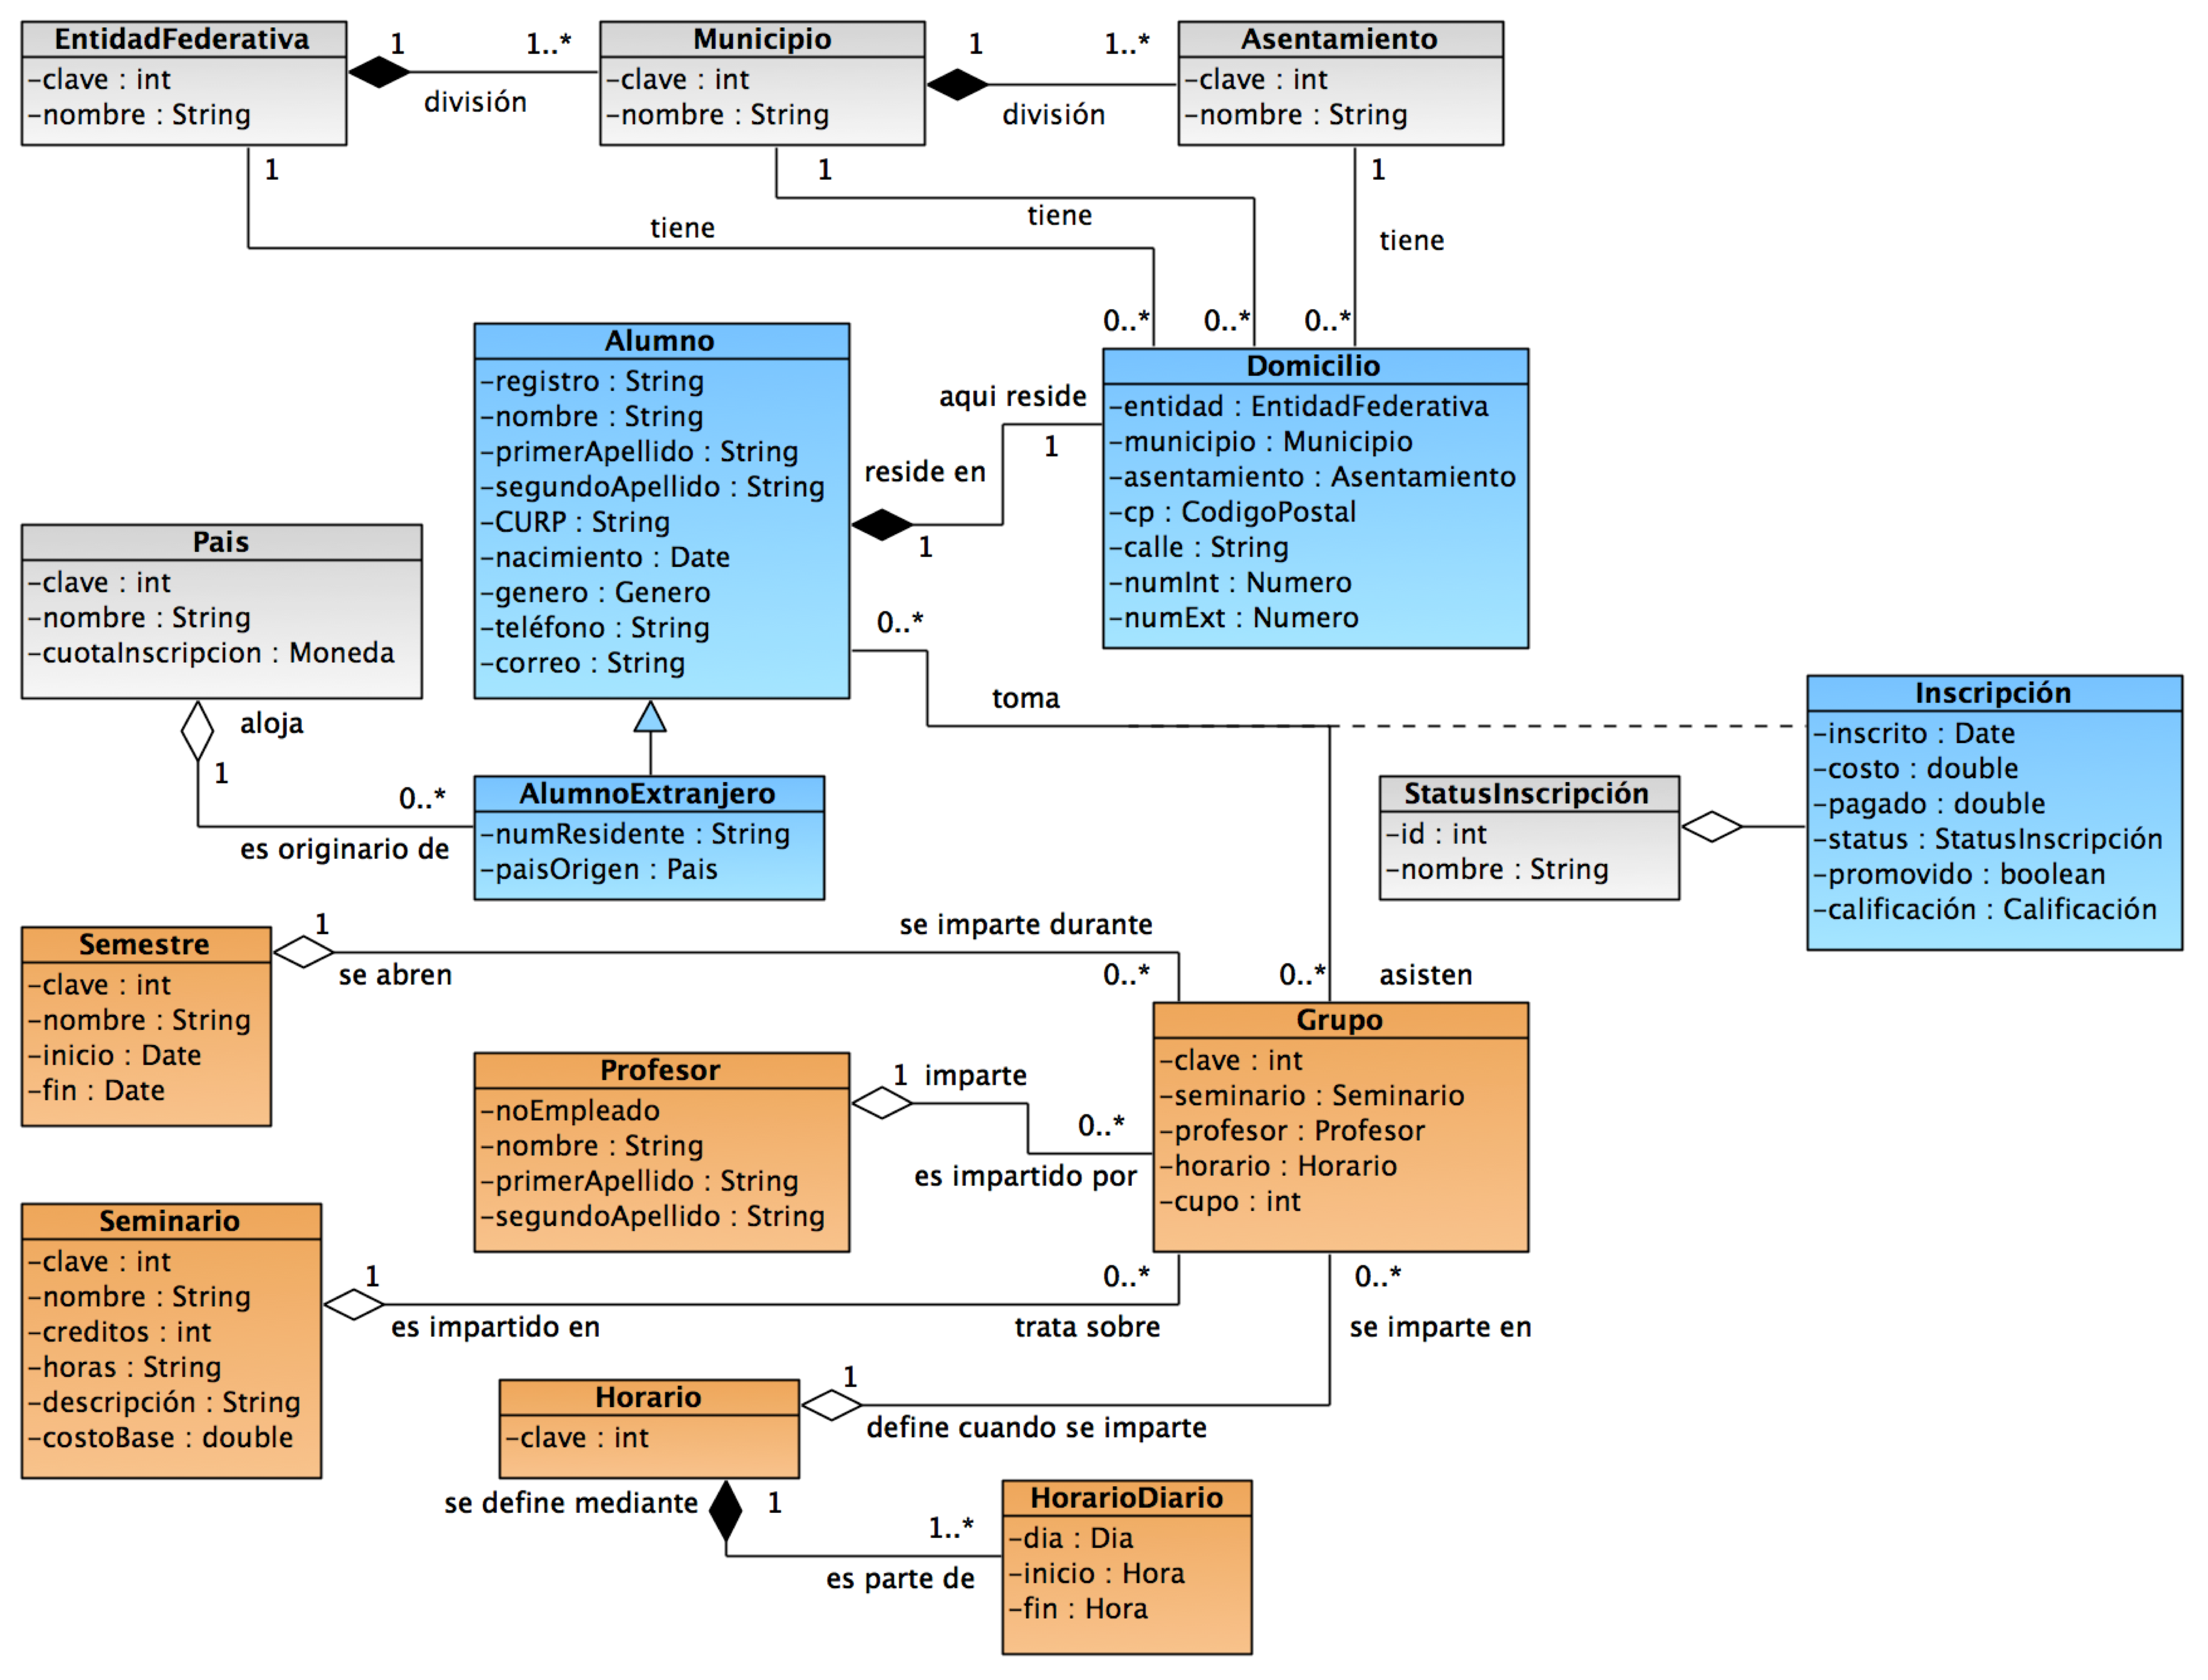
\includegraphics[angle=90,width=.95\textwidth]{images/modeloDelDominioDelProblema}
		\caption{Modelo del dominio del problema}
		\label{fig:modeloDeDominio}
	\end{center}
\end{figure}

\begin{cdtEntidad}{Alumno}{Alumno}
	\brAttr{registro}{Registro}{Id}{Número de registro utilizado para identificar un alumno}{Sí}
	\brAttr{nombre}{Nombre}{Palabra Corta}
		{Nombre o nombres del alumno.}{Sí}
	\brAttr{primerApellido}{Primer apellido}{Palabra Corta}
		{Primer apellido del alumno.}{Sí}
	\brAttr{segundoApellido}{Segundo apellido}{Palabra Corta}
		{Segundo apellido del alumno.}{No}
	\brAttr{CURP}{CURP}{CURP}
		{CURP del alumno.}{Sí}
	\brAttr{nacimiento}{Nacimiento}{Fecha}
		{Fecha de nacimiento del alumno.}{Sí}
	\brAttr{genero}{Género}{Domicilio}
		{Género del alumno.}{No}
	\brAttr{telefono}{Teléfono}{Telefono}
		{Teléfono para contactar al alumno.}{Sí}
	\brAttr{correo}{Correo}{Correo}
		{Correo del alumno para enviar información académica y escolar y para recuperación de clave de acceso.}{Sí}
	\cdtEntityRelSection
	\brRel{\brRelComposition}{Domicilio}{Un \hyperlink{Alumno}{Alumno} reside en un \hyperlink{Domicilio}{Domicilio}}	
	\brRel{\brRelAgregation}{Grupo}{Un \hyperlink{Alumno}{Alumno} toma un \hyperlink{Curso}{Curso}}	
\end{cdtEntidad}

%- - - - - - - - - - - - - - - - - - - - - - - - - - - - - 
\begin{cdtEntidad}{AlumnoExtranjero}{Alumno Extranjero}%{}
	\brAttr{numeroResidente}{Numero de residente}{Id}{Número de registro dado por la Secretaría de Relaciones Exteriores a los extranjeros.}{Si}
	\brAttr{paisOrigen}{Pais origen}{\hyperlink{Pais}{País}}
		{País de origen del alumno extranjero.}{Sí}
	\cdtEntityRelSection
	\brRel{\brRelAgregation}{País}{Un \hyperlink{Alumno}{Alumno} es originario de un \hyperlink{Pais}{Pais}}	
	\brRel{\brRelGeneralization}{Alumno}{Un \hyperlink{AlumnoExtranjero}{Alumno Extranjero} es un  \hyperlink{Alumno}{Alumno}}	
	\brRel{\brRelParticipation}{Alumno}{Un \hyperlink{AlumnoExtranjero}{Alumno Extranjero} es un  \hyperlink{Alumno}{Alumno}}	
\end{cdtEntidad}

%---------------------------------------------------------
\section{Modelado de Reglas de negocio}


% !TeX root = proyecto.tex


\cdtInstrucciones{En esta sección describa todas las reglas de negocio identificadas.}


% Tipo: \btDerivation (no aplica Clase), \btEnabler, \btTimer, \btExecutive
% Clase: \bcCondition, \bcIntegrity, \bcAutorization.
% Cumplimiento: \blStrict \blDeferred \blPreAutorized \blPostJustified \blOverride \blGuideline
\begin{BussinesRule}[%
	\brClassification{\btEnabler}{\bcCondition}{\blStrict}
	]{BR-001}{Nombre de la regla de negocio}
	
				% Opciones para nivel: \blControlling, \blInfluencing
	\BRitem[Descripción:] Descripción de la regla. Forma coloquial a manera de reglamento.
	\BRitem[Motivación:] Describa por que es importante la regla.
	\BRitem[Sentencia:] Sentencia formal de la regla.
	\BRitem[Ejemplo positivo:] Indique uno o varios ejemplos en donde la regla se cumple.
        \begin{itemize}
        	\item ...
        \end{itemize}
	
	\BRitem[Ejemplo negativo:] Indique uno o varios ejemplos en dónde la regla no se cumple.
		\begin{itemize}
        	\item ...
        \end{itemize}
	
	\BRitem[Referenciado por:] Liste los casos de uso en donde la regla no se cumple. por ejemplo \hyperlink{CUCE3.2}{CUCE3.2}, \hyperlink{CUCE3.3}{CUCE3.3}.
\end{BussinesRule}




\section{Máquinas de estado}

% !TeX root = proyecto.tex

\cdtInstrucciones{En esta sección describa para cada máquina de estados y a que entidad corresponde. Utilice reglas ECA en el diagrama y elabore el diagrama de estados, una descripción del diagrama, una descripción de cada estado y una descripción de las acciones indicando que casos de uso están involucrados.}

% - - - - - - - - - - - - - - - - - - - - - - - - - - - - 
\subsection{Estados para un préstamo}

En la figura~\ref{fig:edos-prestamo} se muestran ...

\begin{figure}[htbp]
	\begin{center}
		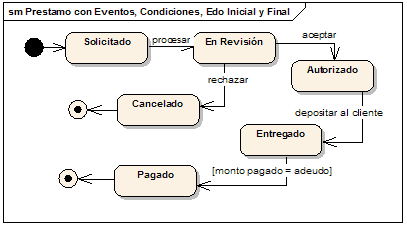
\includegraphics[width=.7\textwidth]{images/edoPrestamo}
		\caption{Máquina de estados de un Préstamo.}
		\label{fig:edos-prestamo}
	\end{center}
\end{figure}

\subsubsection{Estados}

\begin{description}
	\item[Estado:] Descripción del estado.
	\item[...] ...
\end{description}


\subsubsection{Acciones}

\begin{description}
	\item[Acción:] Descripción de la acción indicando el Caso de uso involucrado.
	\item[...] ...
\end{description}






%=========================================================
% !TeX root = proyecto.tex

%=========================================================
\chapter{Modelo dinámico}	
\label{cap:modDinamico}

\cdtInstrucciones{Presente la solución indicando el si esta se compone de varios sistemas, los subsistemas del sistema y si aplica, los módulos de los subsistemas.}

	Este capítulo describe en modelo dinámico del sistema. en el se detallan todos los escenarios de ejecución del sistema. La figura~\ref{fig:casosDeUso} muestra el diagrama general del sistema y sus subsistemas, y la figura~\ref{fig:casosDeUsoDetalle} muestra todos los casos de uso del sistema. En este documento solo detallamos los casos de uso del subsistema de gestión de cursos.
	
\begin{figure}[htbp]
	\begin{center}
		\fbox{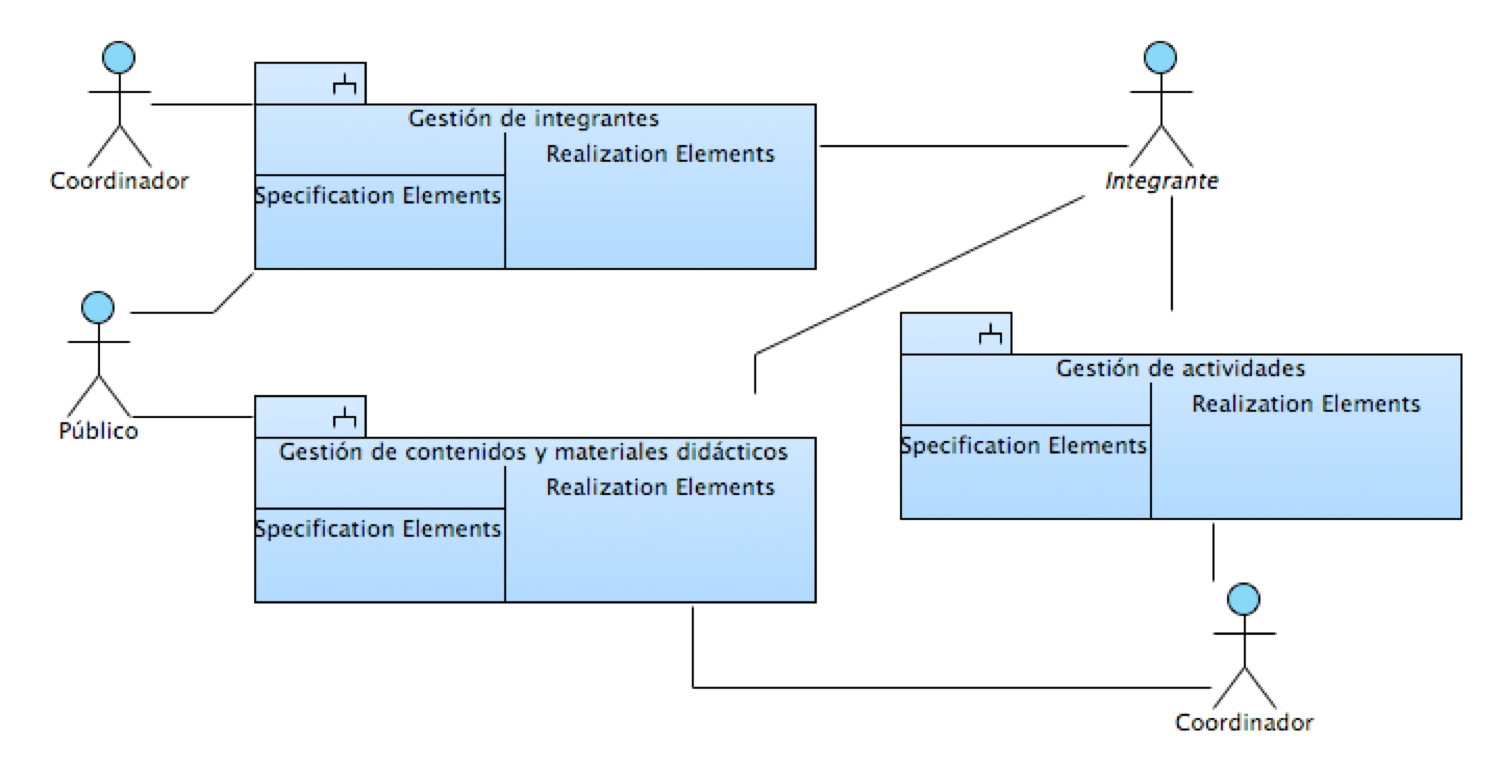
\includegraphics[width=.8\textwidth]{images/casosDeUso}}
		\caption{Diagrama de casos de uso del sistema.}
		\label{fig:casosDeUso}
	\end{center}
\end{figure}

\begin{figure}[htbp]
	\begin{center}
		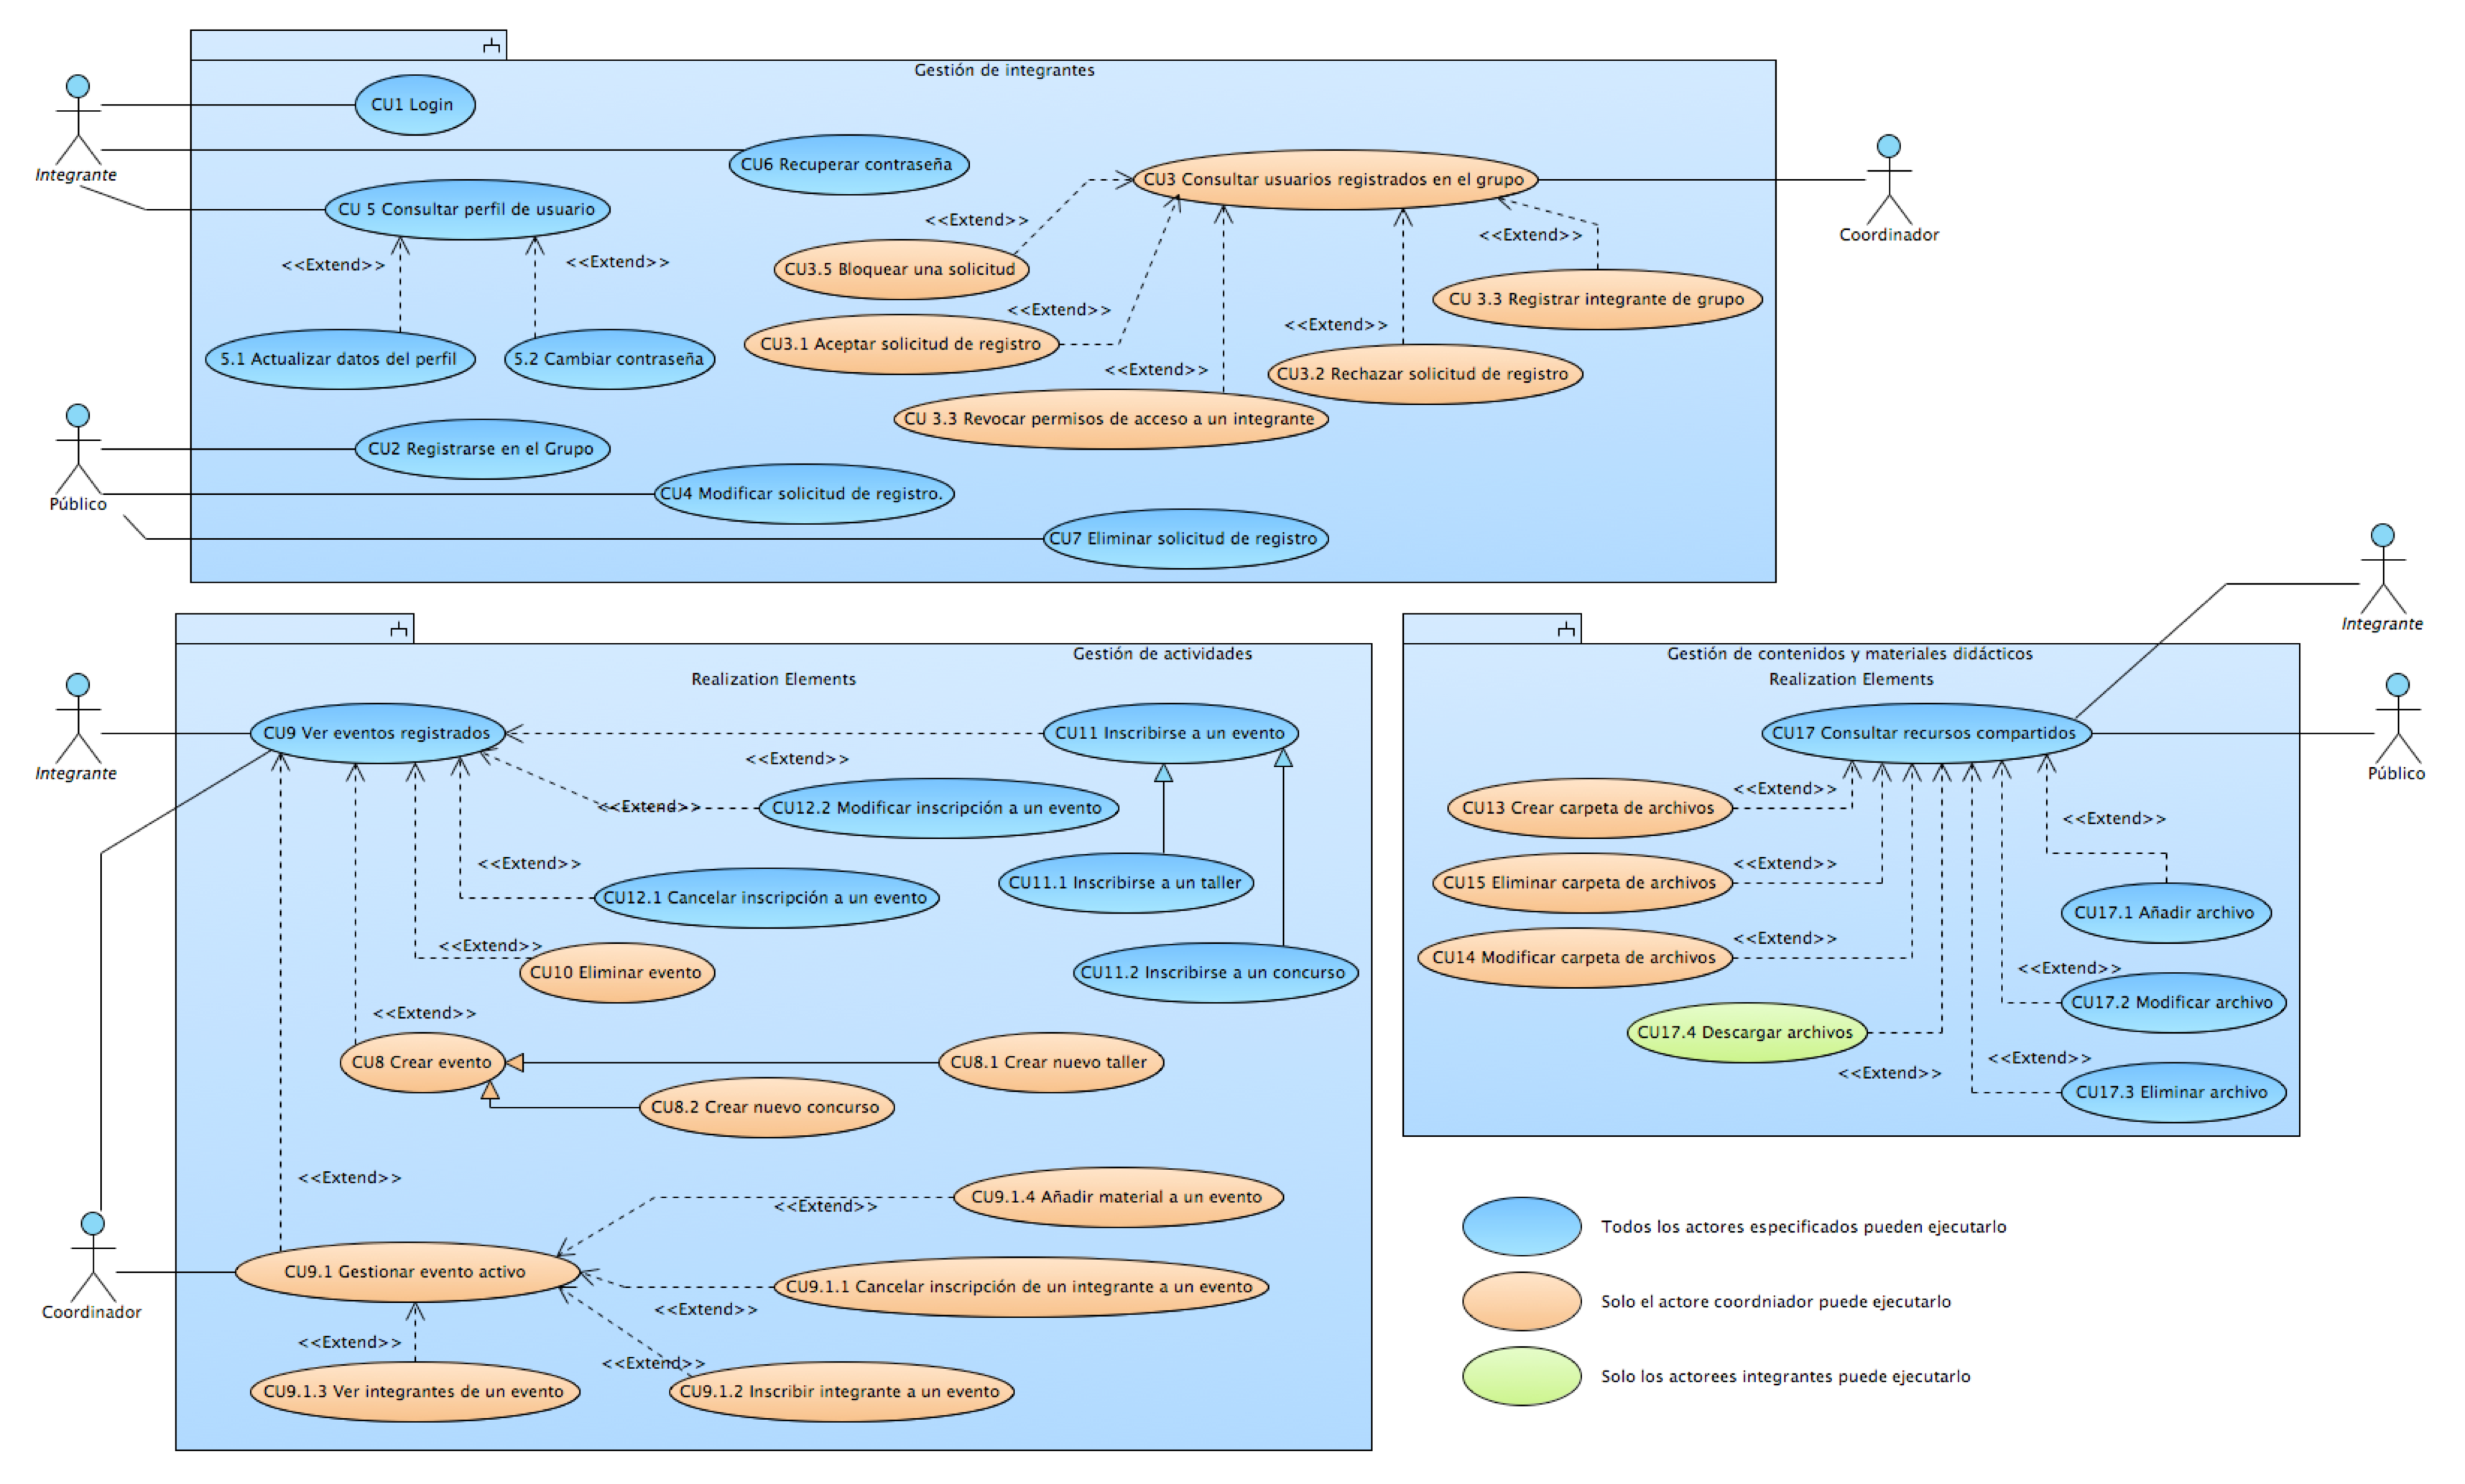
\includegraphics[angle=90, width=.7\textwidth]{images/casosDeUsoDetalle}
		\caption{Diagrama detallado del sistema.}
		\label{fig:casosDeUsoDetalle}
	\end{center}
\end{figure}

%---------------------------------------------------------
\section{Descripción de casos de uso}



A continuación se detallan los casos de uso.

%---------------------------------------------------------
% CASOS DE USO

%!TEX root = ../proyecto.tex

% Plantilla para caso de uso sencillo con ejemplos de comandos e intrucciones.
%-------------------------------------- COMIENZA descripción del caso de uso.

%\begin{UseCase}[archivo de imágen]{UCX}{Nombre del Caso de uso}{
%--------------------------------------
\begin{UseCase}{CUX}{Escriba el nombre del caso de uso}{
	% La descripción debe describir el evento de inicio del caso de uso, Breve descripción de la trayectoria y estado final del caso de uso.
}
	\UCitem{Versión}{\color{Gray}
		0.1	% Ponga un número de versión, 
	}\UCitem{Autor}{\color{Gray}
		Nombre del analista. % Analista responsable de especificar el CU
	}\UCitem{Supervisa}{\color{Gray}
		Nombre del analista revisor. % Analista responsable de verificar que está correcto.
	% TODO: Dar de alta al actor Usuario
	}\UCitem{Actor}{
		\hyperlink{IdDelActor}{Nombre del actor} % No olvide dar de alta el actor.
	}\UCitem{Propósito}{\begin{Titemize}%Indique los fines, objetivos, propósitos o valores agregados del Caso de uso.
		\Titem Propósito del caso de uso.
		\Titem ...
	\end{Titemize}
	}\UCitem{Entradas}{\begin{Titemize}
		% TODO: Dar de alta las entidades que se listan.
		\Titem \hyperlink{Entidad.Atributo}{Nombre del dato de entrada}. % El identificador no acepta acentos, espacios ni eñes.
		\Titem \hyperlink{Entidad.Atributo}{Nombre del dato de entrada}. % Liste todos los datos de entrada
		\end{Titemize}
	}\UCitem{Origen}{\begin{Titemize}
		\Titem Se introducen desde el teclado. % Indique por que medio se introducen los datos, 
		\Titem otros.          % Si es ḿas de uno indique que datos corresponden en cada medio de entrada.
	\end{Titemize}
	}\UCitem{Salidas}{\begin{Titemize}
		% TODO: Dar de alta las entidades que se listan.
		\Titem \hyperlink{Entidad.Atributo}{Nombre del dato de entrada}.
		\Titem Mensajes de error. % Indique por que medio se introducen los datos, 
		\Titem Datos que aparecen en pantalla.          % Si es ḿas de uno indique que datos corresponden en cada medio de entrada.
		\Titem Datos que aparecen en listas desplegables o tablas, etc.
		\Titem Datos que se imprimen o que se envía a otros sistemas.
	\end{Titemize}
	}\UCitem{Destino}{\begin{Titemize}
		\Titem Se muestra en la pantalla \IUref{IUX}{Nombre pantalla}.. % Indique por que medio se muestran los datos, 
		\Titem otros.          % Si es ḿas de uno indique que datos corresponden en cada medio de entrada.
	\end{Titemize}
	}\UCitem{Precondiciones}{\begin{Titemize}
		% Incluya Precondiciones lógicas, de negocio e incluso las que debe atender el usuario. 
		% Muchas precondiciones provienen de reglas de negocios, otras estarán asociadas a manejo de errores
		% Otras están relacionadas con casos de uso que deben ejecutarse previamente, como registrar un producto.
		\Titem Escriba la precondición.
	\end{Titemize}
	}\UCitem{Postcondiciones}{\begin{Titemize}
		% Indique todas las postcondiciones
		% por ejemplo, Cambios en el sistema
		% Cambios en la BD una vez terminado el CU
		% Efectos colaterales
		% Condiciones de término.
		\Titem Escriba todas las postcondiciones.
	\end{Titemize}
	}\UCitem{Errores}{\begin{Titemize}
		% Escriba todos los errores que puedan ocurrir en el sistema, para cada error recuerde:
		% Punerle un identificador
		% Describir la condición o escenario que detona el error
		% Describa la forma en que debe reaccionar el sitema: si la reaccion corresponde a varios pasos use mejor una trayectoria alternativa.
		% Relacione el error con la trayectoria principal.
		\Titem {\bf \hypertarget{CUX.E1}{E1}}: Condición que detona el error, reacción del sistema y regresa al paso \ref{UC1.etiqueta}.
		\Titem {\bf \hypertarget{CUX.E2}{E2}}: Condición que detona el error, reacción del sistema y termina el Caso de uso..
	\end{Titemize}
	}\UCitem{Tipo}{
		% Especifique el tipo de caso de us, puede ser: "Caso de uso primario" o 
		% "Viene de \\hyperref{CUY}{CUY nombre del CU}" cuando se desprende desde otro caso de uso mediante un extends.
		Caso de uso primario
	}\UCitem{Observaciones}{
		% Indique las observaciones al caso de uso, las cuales pueden ser:
		% - Ninguna
		% - Dudas sobre el procedimiento o la especificación.
		% - Issues detectados
		% - Suposiciones realizadas.
		% - Cualquier otra especificacion que considere pertinente que no pudo colocarse en los demás atributos del Caso de uso
		% - Aclaraciones.
		% - Notas para el usuario o desarrollador.
		% - Pendientes (TODO's) en caso de no usar los comentarios.
	}
\end{UseCase}

%--------------------------------------
\begin{UCtrayectoria}
	% Cada paso debe inicair con un Verbo en infinitivo, siempre especificando el objetivo del paso mas la accion en concreto.
	% \UCpaso[\UCactor] se refiere al actor y \UCpaso se refiere al sistema.
	% A continuación viene ejemplos de pasos:
	% En el siguiente paso: "Ingresa al sistema" es el objetivo del paso y "escribiendo la URL de la aplicación" es la acción en concreto.
	\UCpaso[\UCactor o \UCsist] VERBO EN INFINITIVO + (Acción del usuario) + (Acción dentro del sistema)
	\UCpaso[\UCactor] Ingresa al sistema escribiendo la URL de la aplicación.
	% En el siguinte paso se referencia una Interfaz:
	\UCpaso Solicita al usuario que se identifique mediante la pantalla \IUref{IU1}{Inicio de sesión}
	% En el siguiente paso está etiquetado para ser referenciado por un error o trayectoria alternativa:
	\UCpaso[\UCactor] \label{UCX.introduceDatos} Se identifica introduciendo su nombre de usuario y contraseña.
	% En el siguiente paso se usa el comando \IUbutton 
	\UCpaso[\UCactor] Solicita el ingreso al sistema presiona el botón \IUbutton{Ingresar}.
	% En el siguiente paso se referencía un error.
	\UCpaso Busca los datos del usuario identificado por el nombre de usuario introducido \ErrorRef{CUX}{E1}{No hay usuario}
	% En el siguiente paso se señala una trayectoria alternativa
	\UCpaso Verifica que el usuario especificado no esté inactivo \ErrorRef{CUX}{E2}{Usuario inactivo} \Trayref{CUX}{A}.
	% En el siguiente paso se referencían dos errores y una trayectoria alternativa.
	\UCpaso Verifica que la contraseña ingresada coincida con la almacenada \ErrorRef{CUX}{E3}{La contraseña no coincide}\Trayref{CUX}{B}.
	% En el siguiente paso se señala la incusión de otro CU
	\UCpaso[] Se ejecutan los pasos del caso de uso \UCref{CUY}{Nombre del caso de uso}.
	% En el siguiente paso se señala un mensaje.
	\UCpaso Muestra la pantalla \IUref{IU2}{Principal} con el mensaje \MSGref{MSG-001}{Bienvenida al usuario}.
\end{UCtrayectoria}


%--------------------------------------
% Las trayectorias alternativas se identifican con Letras: A, B, C, etc.
\begin{UCtrayectoriaA}{CUX}{LETRA}{Condición que hace que se ejecute esta trayectoria}
	\UCpaso Especifique los pasos  de la trayectoria.
	% Se puede desprender otra trayectria alternativa si es necesario.
	% Finalice la trayectoria indicando si la ejecución se integra a la trayectoria anterior o si termina la ejecución del CU.
	% Verifique que la redacción de la trayectoria deje en claro si el objetivo del CU se alcanzó o no.
	\UCpaso[] El Caso de Uso continúa en el paso \ref{UCX.introduceDatos}.
\end{UCtrayectoriaA}


%--------------------------------------
% Puntos de extensión

% Comente la siguiente sección en caso de que no hayan puntos de extensión o relaciones de tipo extends.
\subsection{Puntos de extensión}
\UCExtenssionPoint{
	% Cuando se dá la extensión del Caso de uso:
	El usuario no recuerda cual es su contraseña o sospecha que su usuario está bloqueado.
}{
	% Durante la región (en que pasos se puede dar la extensión):
	Del paso \ref{CUX.etiqueta} al paso \ref{CUX.etiqueta}.
}{
	% Casos de uso a los que extiende:
	\UCref{CUZ}{Nombre del caso de uso}.
}
		
		
		
%-------------------------------------- TERMINA descripción del caso de uso.
%!TEX root = ../proyecto.tex

% Plantilla para caso de uso sencillo con ejemplos de comandos e intrucciones.
%-------------------------------------- COMIENZA descripción del caso de uso.

%\begin{UseCase}[archivo de imágen]{UCX}{Nombre del Caso de uso}{
%--------------------------------------
\begin{UseCase}{CUX}{Escriba el nombre del caso de uso}{
	% La descripción debe describir el evento de inicio del caso de uso, Breve descripción de la trayectoria y estado final del caso de uso.
}
	\UCitem{Versión}{\color{Gray}0.1}% Ponga un número de versión, 
	\UCitem{Estatus}{\color{Gray}.}
	\UCitem{Prioridad}{\color{Gray}.}
	\UCitem{Usuario}{\color{Gray}Nombre del usuario o usuarios} % Usuarios que dieron la información para el CU.
	\UCitem{Elaboró}{\color{Gray}Nombre del analista} % Analista responsable de especificar el CU
	\UCitem{Supervisó}{\color{Gray}Nombre del analista revisor.} % Analista responsable de verificar que está correcto.
	\UCitem{Validó}{\color{Gray}Nombre del usuario o usuarios} % Usuarios que validan con su firma el caso de uso para su programación.
	\UCitem{Complejidad}{\color{Gray}.} % Muy alta, Alta, Media, Baja, Muy baja.
	\UCitem{Volatilidad}{\color{Gray}.} % Muy alta, Alta, Media, Baja, Muy baja.
	\UCitem{Madurez}{\color{Gray}.} % Muy alta, Alta, Media, Baja, Muy baja.
	\UCitem{Dificultades}{\color{Gray}
		\begin{Titemize}
			% Listar todas las dificultades que tiene el CU o moner la palabra ninguna.
			\Titem 
		\end{Titemize}
	}
	\UCitem{Proceso}{} % ID y nombre del proceso
	\UCitem{Sub-proceso}{} % ID y nombre del subproceso
	\UCitem{Área}{} % Nombre del área a la que oertenece el actor.
	% TODO: Dar de alta al actor Usuario
	\UCitem{Actor}{\hyperlink{IdDelActor}{Nombre del actor}} % No olvide dar de alta el actor.
	\UCitem{Tipo de operación}{} % Consulta, alta, baja, cambio, reporte, operacion del negocio, etc.
	\UCitem{Frecuencia}{ % Con que frecuencia o periodicidad minimá, promedio y máxima se ejecutará este caso de uso en el sistema
		\begin{Titemize}
			\Titem Mínimo:
			\Titem Promedio:
			\Titem Máximo:
		\end{Titemize}
	}
	\UCitem{Volumen}{ % Volumen mínimo, promedio y máximo de usuarios simultaneos o información se podría tener en la presente operación.
		\begin{Titemize}
			\Titem Mínimo:
			\Titem Promedio:
			\Titem Máximo:
		\end{Titemize}
	}
	\UCitem{Req. de usuario}{} % id y nombre de los requerimientos que satisface el CU.
	\UCitem{Fuentes}{
		\begin{Titemize}
			% Lista de fuentes documetnales que respaldan o en los que se basa el Caso de uso.
			\Titem 
		\end{Titemize}
	}	
	\UCitem{Propósito}{
		%Indique el fin, objetivo, propósito o valor agregado del Caso de uso.
		\begin{Titemize}
			\Titem 
		\end{Titemize}
	}
	\UCitem{Entradas}{
		\begin{Titemize}
			% TODO: Dar de alta las entidades que se listan.
			\Titem \hyperlink{Entidad.Atributo}{Nombre del dato de entrada}. % El identificador no acepta acentos, espacios ni eñes.
			\Titem \hyperlink{Entidad.Atributo}{Nombre del dato de entrada}. % Liste todos los datos de entrada
		\end{Titemize}
	}
	\UCitem{Origen}{\begin{Titemize}
			\Titem Se introducen desde el teclado. % Indique por que medio se introducen los datos, 
			\Titem otros.          % Si es ḿas de uno indique que datos corresponden en cada medio de entrada.
		\end{Titemize}} 
	\UCitem{Salidas}{\begin{Titemize}
			% TODO: Dar de alta las entidades que se listan.
			\Titem \hyperlink{Entidad.Atributo}{Nombre del dato de entrada}.
			\Titem Mensajes de error. % Indique por que medio se introducen los datos, 
			\Titem Datos que aparecen en pantalla.          % Si es ḿas de uno indique que datos corresponden en cada medio de entrada.
			\Titem Datos que aparecen en listas desplegables o tablas, etc.
			\Titem Datos que se imprimen o que se envía a otros sistemas.
	\end{Titemize}}
	\UCitem{Destino}{\begin{Titemize}
			\Titem Se muestra en la pantalla \IUref{IUX}{Nombre pantalla}.. % Indique por que medio se muestran los datos, 
			\Titem otros.          % Si es ḿas de uno indique que datos corresponden en cada medio de entrada.
	\end{Titemize}}
	\UCitem{Disparadores}{
	\begin{Titemize}
		% Liste y describa los escenarios en los que el actor debe ejecutar el caso de uso
		\Titem 
	\end{Titemize}
	}
	\UCitem{Precondiciones}{
		\begin{Titemize}
			% Incluya Precondiciones lógicas, de negocio e incluso las que debe atender el usuario. 
			% Muchas precondiciones provienen de reglas de negocios, otras estarán asociadas a manejo de errores
			% Otras están relacionadas con casos de uso que deben ejecutarse previamente, como registrar un producto.
			\Titem Escriba la precondición.
		\end{Titemize}
	}
	\UCitem{Condición de término}{
	\begin{Titemize}
		% Liste todos los efectos que un usuario (aunque sea otro actor) puede o debe ver en el sistema 
		% como consecuencia de la ejecución del cao de uso.
		\Titem 
	\end{Titemize}
	}
	\UCitem{Efectos colaterales}{
	\begin{Titemize}
		% 
		\Titem 
	\end{Titemize}
	}
	\UCitem{Postcondiciones}{
		\begin{Titemize}
			% Indique todas las postcondiciones que no haya listado en efectos colaterales o condiciones de término.
			% por ejemplo, Cambios en el sistema
			% Cambios en la BD una vez terminado el CU
			\Titem Escriba todas las postcondiciones.
		\end{Titemize}
	}
	\UCitem{Errores}{
		% Escriba todos los errores que puedan ocurrir en el sistema, para cada error recuerde:
		% Punerle un identificador
		% Describir la condición o escenario que detona el error
		% Describa la forma en que debe reaccionar el sitema: si la reaccion corresponde a varios pasos use mejor una trayectoria alternativa.
		% Relacione el error con la trayectoria principal.
		\begin{Titemize}
			\Titem {\bf \hypertarget{CUX.E1}{E1}}: Condición que detona el error, reacción del sistema y regresa al paso \ref{UC1.etiqueta}.
			\Titem {\bf \hypertarget{CUX.E2}{E2}}: Condición que detona el error, reacción del sistema y termina el Caso de uso..
		\end{Titemize}
	}
	\UCitem{Tipo}{
		% Especifique el tipo de caso de us, puede ser: "Caso de uso primario" o 
		% "Viene de \\hyperref{CUY}{CUY nombre del CU}" cuando se desprende desde otro caso de uso mediante un extends.
		Caso de uso primario
	}
	\UCitem{Casos de prueba}{
		% Liste todos los casos de prueba que identifica.
		\begin{Titemize}
			\Titem {\bf \hypertarget{CUX.E1}{E1}}: Condición que detona el error, reacción del sistema y regresa al paso \ref{UC1.etiqueta}.
			\Titem {\bf \hypertarget{CUX.E2}{E2}}: Condición que detona el error, reacción del sistema y termina el Caso de uso..
		\end{Titemize}
	}
	\UCitem{Consideraciones de diseño}{
	% Consideraciones tales como tiempo máximo de respuesta, retroalimentación, animaciones, cálculos complejos, operaciones asíncronas, etc.
	\begin{Titemize}
		\Titem ...
	\end{Titemize}
	}\UCitem{Impedimentos}{
	% Liste todos los impedimentos que conozca sobre este caso de uso
	\begin{Titemize}
		\Titem {\bf \hypertarget{CUX.E1}{E1}}: Condición que detona el error, reacción del sistema y regresa al paso \ref{UC1.etiqueta}.
		\Titem {\bf \hypertarget{CUX.E2}{E2}}: Condición que detona el error, reacción del sistema y termina el Caso de uso..
	\end{Titemize}
	}\UCitem{Preguntas}{
	% Liste todas las preguntas no contestadas del caso de uso
	\begin{Titemize}
		\Titem ...
	\end{Titemize}
	}\UCitem{Observaciones}{
		% Indique las observaciones al caso de uso, las cuales pueden ser:
		% - Ninguna
		% - Dudas sobre el procedimiento o la especificación.
		% - Issues detectados
		% - Suposiciones realizadas.
		% - Cualquier otra especificacion que considere pertinente que no pudo colocarse en los demás atributos del Caso de uso
		% - Aclaraciones.
		% - Notas para el usuario o desarrollador.
		% - Pendientes (TODO's) en caso de no usar los comentarios.
	}
\end{UseCase}

%--------------------------------------
\begin{UCtrayectoria}
	% Cada paso debe inicair con un Verbo en infinitivo, siempre especificando el objetivo del paso mas la accion en concreto.
	% \UCpaso[\UCactor] se refiere al actor y \UCpaso se refiere al sistema.
	% A continuación viene ejemplos de pasos:
	% En el siguiente paso: "Ingresa al sistema" es el objetivo del paso y "escribiendo la URL de la aplicación" es la acción en concreto.
	\UCpaso[\UCactor] Ingresa al sistema escribiendo la URL de la aplicación.
	% En el siguinte paso se referencia una Interfaz:
	\UCpaso Solicita al usuario que se identifique mediante la pantalla \IUref{IU1}{Inicio de sesión}
	% En el siguiente paso está etiquetado para ser referenciado por un error o trayectoria alternativa:
	\UCpaso[\UCactor] \label{UCX.introduceDatos} Se identifica introduciendo su nombre de usuario y contraseña.
	% En el siguiente paso se usa el comando \IUbutton 
	\UCpaso[\UCactor] Solicita el ingreso al sistema presiona el botón \IUbutton{Ingresar}.
	% En el siguiente paso se referencía un error.
	\UCpaso Busca los datos del usuario identificado por el nombre de usuario introducido 
	% En el siguiente paso se señala una trayectoria alternativa
	\UCpaso Verifica que el usuario especificado no esté inactivo  \Trayref{CUY}{A}.
	% En el siguiente paso se referencían dos errores y una trayectoria alternativa.
	\UCpaso Verifica que la contraseña ingresada coincida con la almacenada \Trayref{CUY}{B}.
	% En el siguiente paso se señala la incusión de otro CU
	\UCpaso[] Se ejecutan los pasos del caso de uso \UCref{CUY}{CUY Nombre del caso de uso}.
	% En el siguiente paso se señala un mensaje.
	\UCpaso Muestra la pantalla \IUref{IU2}{Principal} con el mensaje \hyperlink{MSG1}{MSG1 Bienvenida al usuario}.		
\end{UCtrayectoria}


%--------------------------------------
% Las trayectorias alternativas se identifican con Letras: A, B, C, etc.
\begin{UCtrayectoriaA}{CUY}{LETRA}{Condición que hace que se ejecute esta trayectoria}
	\UCpaso Especifique los pasos  de la trayectoria.
	% Se puede desprender otra trayectria alternativa si es necesario.
	% Finalice la trayectoria indicando si la ejecución se integra a la trayectoria anterior o si termina la ejecución del CU.
	% Verifique que la redacción de la trayectoria deje en claro si el objetivo del CU se alcanzó o no.
	\UCpaso[] El Caso de Uso continúa en el paso \ref{UCX.introduceDatos}.
\end{UCtrayectoriaA}


%--------------------------------------
% Puntos de extensión

% Comente la siguiente sección en caso de que no hayan puntos de extensión o relaciones de tipo extends.
\subsection{Puntos de extensión}
\UCExtenssionPoint{
	% Cuando se dá la extensión del Caso de uso:
	El usuario no recuerda cual es su contraseña o sospecha que su usuario está bloqueado.
}{
	% Durante la región (en que pasos se puede dar la extensión):
	Del paso \ref{CUX.etiqueta} al paso \ref{CUX.etiqueta}.
}{
	% Casos de uso a los que extiende:
	\UCref{CU3.4}{Consultar historial académico}.
}
		
		
		
%-------------------------------------- TERMINA descripción del caso de uso.
%\input{cu/cu-02}
%\input{cu/cu-03}
%\input{cu/cu-04}
%\input{cu/cu-05}
%\input{cu/cu-06}
%\input{cu/cu-07}
%\input{cu/cu-08}




%=========================================================
% !TeX root = proyecto.tex
%=========================================================
\chapter{Modelo de la interacción}	
\label{cap:modInteraccion}

\cdtInstrucciones{Introduzca el capítulo indicando su contenido y organización.}	

\cdtInstrucciones{Utilice este capítulo para describir todos los detalles de la interacción con el usuario, describiendo elementos d eusabilidad, ergonomía, psicología,  arqjuitectura de información y repreentación.}

Este capítulo describe ...

\section{Modelo de navegación}

\cdtInstrucciones{Describa de acuerdo al tipo de aplicación como es la interacción con el usuario, destacando los elementos de ubicación dentro de la aplicación. Si las interfaces tiene elementos comunes más allá de los que son comunes a todas las aplicaciones describalos ampliamente así como los encabezados, pies de página, menús y otros elementos que aparecen repetitivamente entre las pantallas.}

	La navegación entre pantallas se muestra en la figura~\ref{fig:mapa}. en el se explica ...\\

\begin{figure}[htbp]
	\begin{center}
		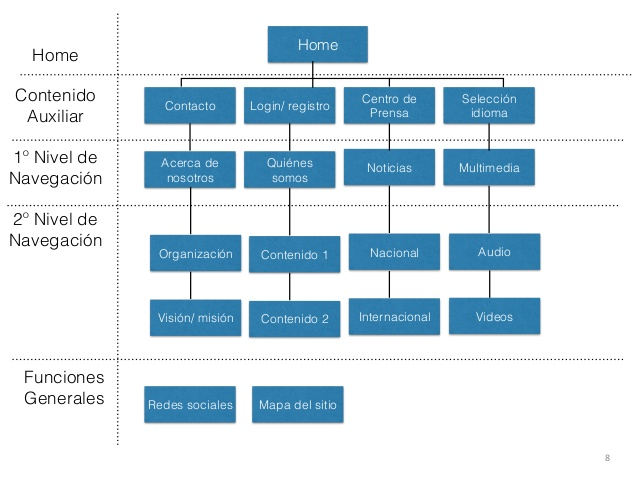
\includegraphics[width=.7\textwidth]{images/mapa}
		\caption{mapa}
		\label{fig:mapa}
	\end{center}
\end{figure}


\cdtInstrucciones{A continuación describa cada una de las pantallas.}
% !TeX root = ../proyecto.tex
%--------------------------------------
\section{IUX Interfaz (nombre de la interfaz)}

\subsection{Objetivo}
	\cdtInstrucciones{Describa el objetivo, propósito o función de la pantalla.}

\subsection{Diseño}
	\cdtInstrucciones{Describa brevemente los elementos de la pantalla y como de be usarse a manera de manual de usuario.} Esta pantalla \IUref{IU23}{Pantalla de Control de Acceso} aparece al iniciar el sistema, para ingresar ... 

\IUfig[.7]{Login}{IU23}{Pantalla de Control de Acceso.}

%\IUfig[ancho de la figura: valor entre 1 y .1]{Nombre corto de la pantalla sin espacions ni acentos}{IUXX}{Nombre largo de la pantalla.}

\subsection{Salidas}

	\cdtInstrucciones{Liste las salidas de la interfaz. Si coinciden con las del caso de uso solo indiquelo. Esta ,ista debe incluir los mensajes}

	\begin{itemize}
		\item Descripción de salida.
	\end{itemize}
	
\subsection{Entradas}

	\cdtInstrucciones{Liste las entradas de la interfaz. Si coinciden con las del caso de uso solo indiquelo.}
	\begin{itemize}
		\item Descripción de salida.
	\end{itemize}

\subsection{Comandos}
	\cdtInstrucciones{Describa cada control (botónes, areas de drag and drop, componentes interactivos, animaciones, etc.) que se puede utilizar dentro de la pantalla indicando o que hacen y si cambia de pantalla.}

\begin{itemize}
	\item \IUbutton{Entrar}: Verifica que el Estudiante se encuentre registrado y la contraseña sea la correcta. Si la verificación es correcta, se muestra la \IUref{UI32}{Pantalla de Selección de Seminario}.
	\item \IUbutton{Ayuda}: Muestra la ayuda de esta pantalla \IUref{IU50}{Pantalla de Ayuda}.
\end{itemize}



%!TEX root = ejemplo.tex
%=========================================================
\section{Catálogo de mensajes}	
\label{sec:mensajes}

	En esta sección se describen todos los mensajes que aparecen en el sistema. Para cada mensaje se especifica:
	 
	\begin{description}\itemsep0em
		\item[Id:] Identificador del mensaje de la forma ``MSG XX'' y descripción corta del mismo.
		\item[Tipo:] Tipo del mensaje el cual puede ser: 
		\begin{description}
			\item[Normal:] Mensaje que informa al usuario una instrucción o el estado interno que guarda el sistema, suele tener un color {\color{msgNormalColor}Azul}.
			\item[Éxito:] Mensaje que informa al usuario sobre una acción realizada, sirve para confirmar el correcto funcionamiento del sistema. Se presentan con un color {\color{msgInfoColor}Verde}.
			\item[Atención:] Mensaje que tiene como finalidad llamar la atención del usuario a una situación que requiere su intervención, por ejemplo cuando una actividad ha generado un efecto colateral o se realizará una acción destructiva y no reversible. Se presentan con un color {\color{msgWarningColor}Naranja}.
			\item[Error:] Mensaje que informa al usuario un fallo en en una operación o un impedimento para realizarla, por ejemplo: cuando no se puede efectuar la acción solicitada, cuando un dato falta o tiene un formato no aceptado por el sistema. Se presentan con un color {\color{msgErrorColor}Rojo}.
		\end{description}
		\item[Propósito:] Explicación del propósito del mensaje.
		\item[Redacción:] Redacción del mensaje.
		\item[Parámetros:] En caso de que el mensaje pueda variar se especifican los casos y la forma en que debe adaptarse la redacción
		\item[Ejemplos:] Ejemplos de como debe renderizarse el mensaje.
	\end{description}


\subsection{Lista de mensajes}

%msgNormalColor
%msgInfoColor
%msgWarningColor
%msgErrorColor
\begin{cdtMessage}[msgInfoColor]{MSG-001}{Bienvenida al usuario}
	\item[Propósito:] Indicar al usuario que ha ingresado satisfactoriamente al sistema.
	\item[Redacción:] Bienvenido $<$nombre$>$.
	\item[Parámetros:] \hspace{1cm}
	\begin{itemize}
		\item $<$nombre$>$ \hyperlink{Usuario.nombre}{Nombre completo} del Usuario.
	\end{itemize}
	\item[Ejemplos:] Bienvenido Juan Pérez.
\end{cdtMessage}

%msgNormalColor
%msgInfoColor
%msgWarninigColor
%msgErrorColor
\begin{cdtMessage}{MSG-002}{Usuario no registrado} 
	\item[Propósito:] Indica que el usuario ingresado no existe en el sistema.
	\item[Redacción:] El usuario $<$login$>$ no se encuentra registrado.
	\item[Parámetros:] \hspace{1cm}
	\begin{itemize}
		\item $<$login$>$ \hyperlink{Usuario.login}{Login} del Usuario.
	\end{itemize}
	\item[Ejemplos:] El usuario juanP no se encuentra registrado.
\end{cdtMessage}

%msgNormalColor
%msgInfoColor
%msgWarninigColor
%msgErrorColor
\begin{cdtMessage}[msgErrorColor]{MSG-003}{Cuenta inactiva} 
	\item[Propósito:] Indicar al usuario que la cuenta especificada se encuentra inactiva.
	\item[Redacción:] La cuenta especificada $<$login$>$ se encuentra inactiva, favor de contactar al Secretario Escolar para mas información.
	\item[Parámetros:] \hspace{1cm}
	\begin{itemize}
		\item $<$login$>$ \hyperlink{Usuario.login}{Login} del Usuario.
	\end{itemize}
	\item[Ejemplos:] La cuenta especificada juanP se encuentra inactiva, favor de contactar al Secretario Escolar para mas información.
\end{cdtMessage}

%msgNormalColor
%msgInfoColor
%msgWarninigColor
%msgErrorColor
\begin{cdtMessage}[msgErrorColor]{MSG-004}{Error de inicio de sesión}
	\item[Propósito:] Indica al usuario que la contraseña introducida es incorrecta.
	\item[Redacción:] La contraseña ingresada es incorrecta.
	\item[Parámetros:] No aplica.
	\item[Ejemplos:] La contraseña ingresada es incorrecta.
\end{cdtMessage}

%msgNormalColor
%msgInfoColor
%msgWarninigColor
%msgErrorColor
\begin{cdtMessage}{MSG-008}{Tiempo restante para terminar un proceso} 
	\item[Propósito:] Indicar al usuario el tiempo restante para terminar una operación limitada en el tiempo como la reinscripción.
	\item[Redacción:] Quedan $<$tiempo$>$ para terminar la $<$operación$>$.
	\item[Parámetros:] \hspace{1cm}
	\begin{itemize}
		\item $<$tiempo$>$ Tiempo faltante para la operació especificando días, horas minutos y segundos.
		\item 
	\end{itemize}
	\item[Ejemplos:] \hspace{1cm}
	\begin{itemize}
		\item Quedan 45 días, 2 horas 12 minutos y 45 segundos para iniciar tu reinscripción.
		\item Quedan 2 minutos y 32 segundos para terminar tu reinscripción
	\end{itemize}
\end{cdtMessage}

\begin{cdtMessage}[msgInfoColor]{MSG-009}{Operación exitosa}
	\item[Propósito:] Informar al usuario que la operación solicitada ha sido ejecutada con éxito.
	\item[Redacción:] $<$Artículo$>$ $<$Operación$>$ del $<$Entidad$>$ $<$Identificador$>$ se realizó con éxito.
	\item[Parámetros:]\hspace{1pt}
	\begin{itemize}
		\item $<$Artículo$>$ $<$Operación$>$ se refiere a la operación realizada.
		\item $<$Entidad$>$ $<$Identificador$>$ se refiere al elemento del negocio donde recayó la operación, indicando el tipo del objeto y un dato que el usuario pueda usar para identificarlo.
	\end{itemize}
	\item[Ejemplo:] Algunos ejemplos son
	\begin{itemize}
		\item El registro del Alumno 342343 se realizó con éxito.
		\item La eliminación de la Tarea ``documentar el proceso'' se ha realizado con éxito.
	\end{itemize}
\end{cdtMessage}


\end{document}
